\section{Equilibri e loro biforcazioni}
Annullando le derivate delle equazioni del sistema, con semplici passaggi si ottengono gli equilibri mostrati in~\autoref{tab:equilibria}.

\begin{table}
    \centering
    \begin{tabular}{l | l}
        \textbf{R} & \textbf{Equilibri}\\
        \hline
        $R \le \dfrac{\strut 1}{\strut\alpha}$ & $(0, 0)$\\
        $R > \dfrac{\strut 1}{\strut\alpha}$ & $(0,0),
        \left( \pm \sqrt{\dfrac{\strut\alpha R -1}{\strut\beta R^3}}, \pm \sqrt{\dfrac{\alpha R -1}{\beta R}} \right)$
    \end{tabular}
    \caption{Equilibri del sistema al variare di $R$.}
    \label{tab:equilibria}
\end{table}

\subsection{Stabilità}
Lo jacobiano del sistema linearizzato è:
\begin{equation}
J(x_1,x_2) =
\begin{bmatrix}
-\dfrac{\strut R}{L\strut} & \dfrac{1}{L} \\
-\dfrac{\strut 1}{C\strut} & \dfrac{\alpha}{C}-\dfrac{\beta}{C} 3x_2^2 \\
\end{bmatrix}
\end{equation}

Analizziamo ora il tipo degli equilibri.
\begin{enumerate}
\item (0,0)\\
\begin{equation}
    J(0,0) =
    \begin{bmatrix}
    -\dfrac{\strut R}{L\strut} & \dfrac{1}{L} \\
    -\dfrac{\strut 1}{C\strut} & \dfrac{\alpha}{C} \\
    \end{bmatrix}
\end{equation}

\begin{equation}
\textrm{tr } J(0,0) = \frac{L\alpha-CR}{CL}
\end{equation}
\begin{equation}
\det J(0,0) = \frac{1-r\alpha}{CL}
\end{equation}
L'analisi di stabilità dell'equilibrio è mostrata in~\autoref{stab-00}.

\item $\left( \pm \sqrt{\dfrac{\strut\alpha R -1}{\strut\beta R^3}}, \pm \sqrt{\dfrac{\alpha R -1}{\beta R}} \right)$

Questi equilibri esistono solo per $R > \frac{1}{\alpha}$, condizione che dunque può essere assunta nello studio della loro stabilità.

\begin{equation}
    J\left( \pm \sqrt{\dfrac{\strut\alpha R -1}{\strut\beta R^3}}, \pm \sqrt{\dfrac{\alpha R -1}{\beta R}} \right) =
    \begin{bmatrix}
        -\dfrac{R\strut}{L\strut} & \dfrac{1}{L} \\
        -\dfrac{1\strut}{C\strut} & \dfrac{3-2R\alpha}{CR} \\
    \end{bmatrix}
\end{equation}

\begin{equation}
    \det J = 2 \dfrac{R\alpha-1}{CL} > 0 \quad \forall R > \frac{1}{\alpha}
\end{equation}

\begin{equation}
    \textrm{tr } J = \dfrac{-CR^2+3L-2RL\alpha}{CRL}
\end{equation}

L'analisi di stabilità degli equilibri è mostrata in~\autoref{stab-eq2}.

\begin{table}
    \centering
    \begin{subtable}[Equilibrio $(0,0)$]{\textwidth}
        \centering
        \begin{tabular}{l l l l l}
            & & tr $J(0,0)$ & $\det J(0,0)$ & tipo\\
            \hline
            $R<\dfrac{1\strut}{\alpha\strut}$ & $(0, 25 \Omega)$ & $>0$ & $>0$ & instabile \\
            \hline
            $\dfrac{1\strut}{\alpha\strut}<R<\dfrac{L\alpha}{C}$ & $(25 \Omega, 40 \Omega)$ & $>0$ & $<0$ & sella \\
            \hline
            $R>\dfrac{L\alpha\strut}{C\strut}$ & $(40 \Omega, +\infty)$ & $<0$ & $<0$ & sella \\
            \hline
        \end{tabular}
        \caption{Stabilità dell'equilibrio $(0,0)$ al variare di R.}
        \label{stab-00}
    \end{subtable}
    \par\bigskip\bigskip
    \begin{subtable}[Equilibrio $(0,0)$]{\textwidth}
        \centering
        \begin{tabular}{l l l l l}
            & & tr $J$ & $\det J$ & tipo\\
            \hline
            $\dfrac{1\strut}{\alpha\strut}<R<k$\tablefootnote{$k=\dfrac{-L\alpha + \sqrt{L^2\alpha^2+3LC}}{C} = 27.82 \Omega$}
            & $(25 \Omega, 27.82 \Omega)$ & $>0$ & $>0$ & fuoco instabile \\
            \hline
            $R>k$ & $(27.82 \Omega, +\infty)$ & $<0$ & $>0$ & fuoco stabile \\
            \hline
        \end{tabular}
        \caption{Stabilità dell'equilibrio $\left( \pm \sqrt{\frac{\alpha R -1}{\beta R^3}}, \pm \sqrt{\frac{\alpha R -1}{\beta R}} \right)$ al variare di R.}
        \label{stab-eq2}
    \end{subtable}
    \caption{Analisi di stabilità degli equilibri (\autoref{tab:equilibria}).}
\end{table}

\subsection{Biforcazioni degli stati di equilibrio}
Le biforcazioni del sistema al variare di $R$ sono elencate in~\autoref{tab:biforc-r}.
Il sistema ammette una biforcazione forcone, due Hopf, una doppia omoclina e una biforcazione tangente di cicli. I valori di $R$ a cui si presentano le biforcazioni doppia omoclina e tangente di cicli sono stati ricavati empiricamente simulando il sistema con Pplane.

\begin{table}
    \centering
    \begin{tabular}{l l p{0.5\linewidth}}
        $\mathbf{R}$ & \textbf{Tipo} & \textbf{Note}\\
        \hline
        $\frac{1}{\alpha} = 25 \Omega$ & forcone & per $R>25 \Omega$ nascono due equilibri instabili (\autoref{fig:forcone}) \\
        \hline
        $k=27.82 \Omega$ & Hopf (doppia) & intorno ai due rami del forcone si creano cicli instabili; i due equilibri diventano stabili (\autoref{fig:hopf}) \\
        \hline
        $28.35 \Omega$ & doppia omoclina & i cicli generati dalle Hopf collidono con la sella in $(0,0)$; si crea un nuovo ciclo instabile interno (\autoref{fig:dopo-omoclina}) \\
        \hline
        $28.49 \Omega$ & tangente di cicli & il ciclo instabile interno e quello stabile esterno collidono e spariscono \\
        \hline
    \end{tabular}
    \caption{Biforcazioni del sistema al variare di $R$.}
    \label{tab:biforc-r}
\end{table}

\begin{figure}
    \centering
    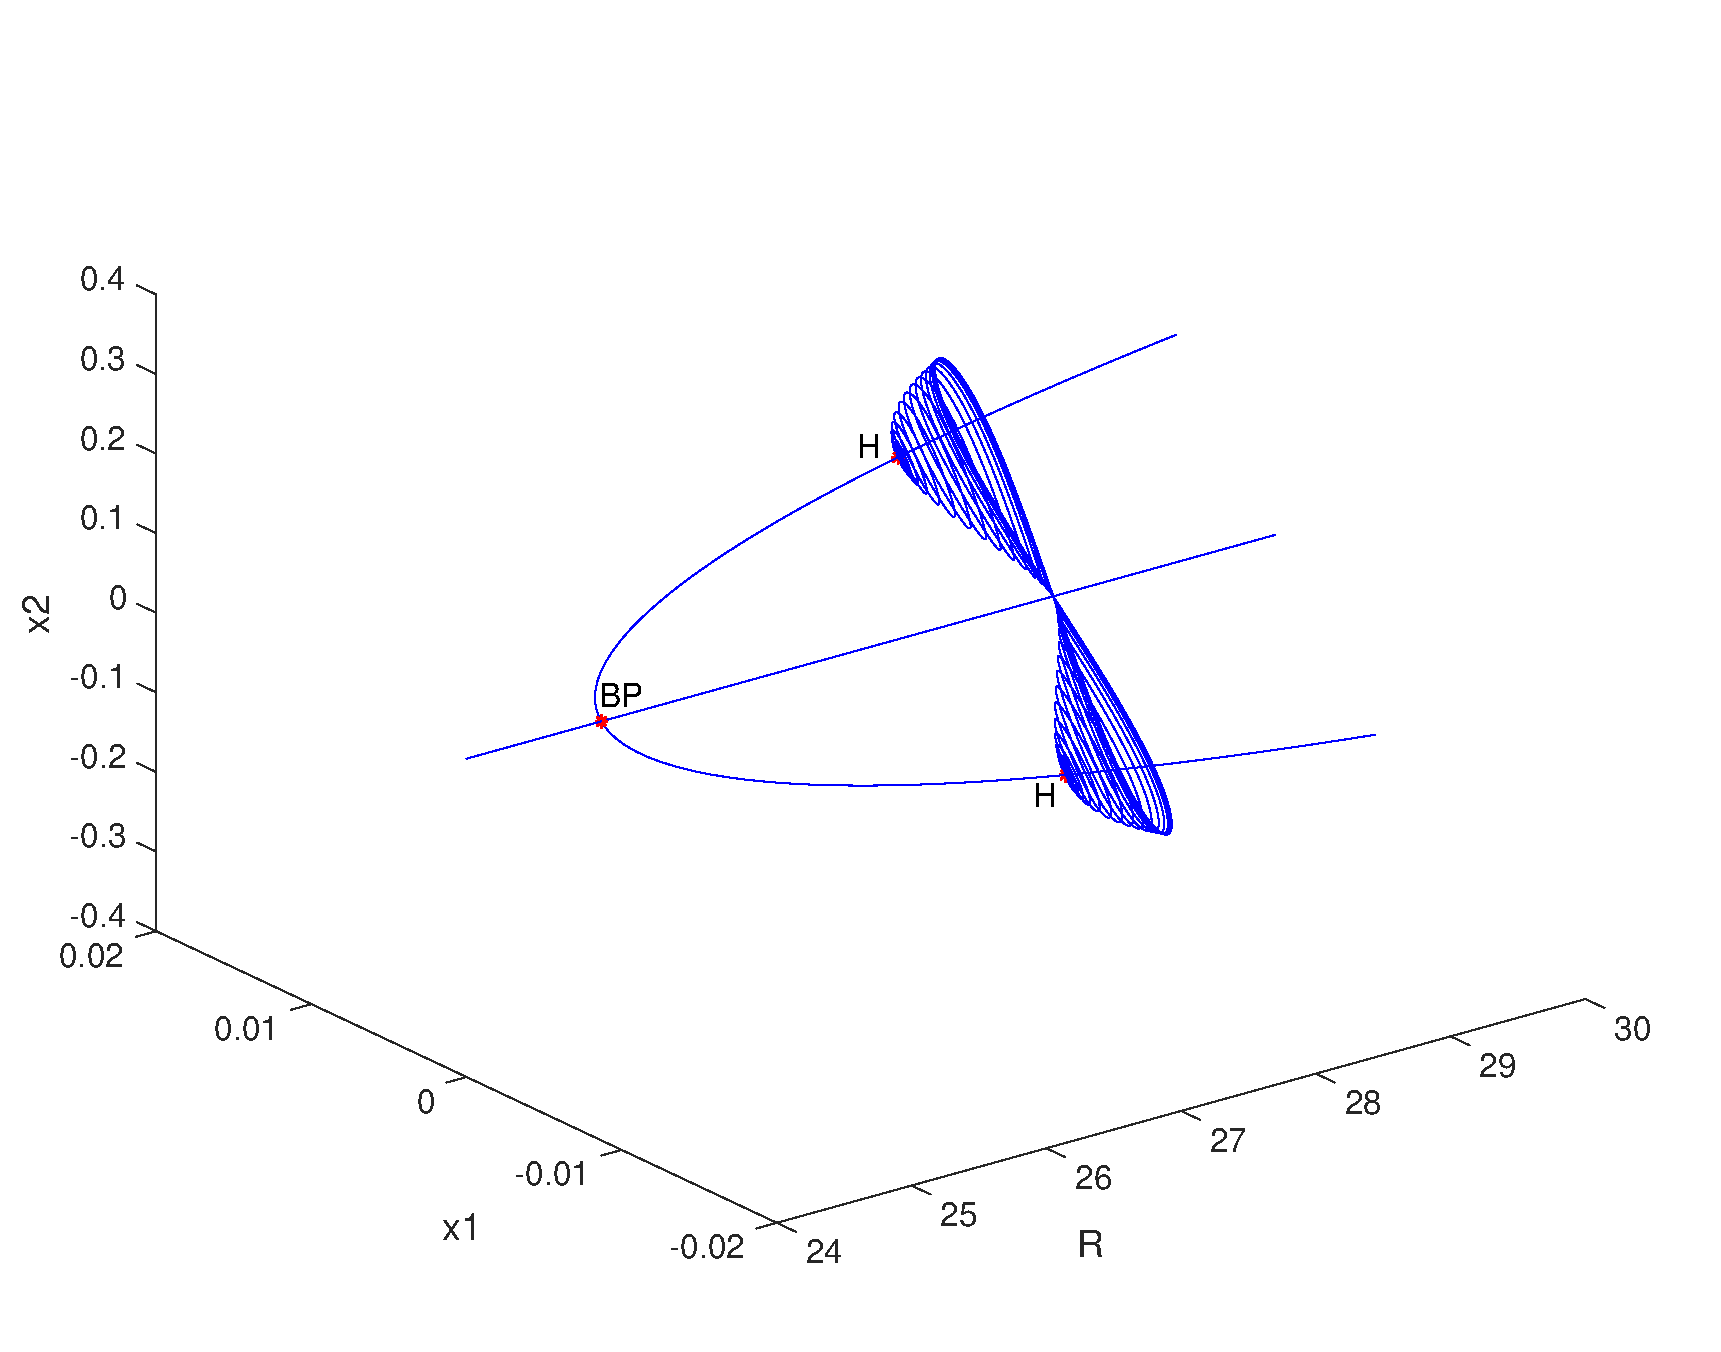
\includegraphics[width=1\textwidth]{matcont/ForconeHopf}
    \caption{Le biforcazioni forcone e Hopf.}
    \label{fig:forcone}
\end{figure}

\subsection{Cicli}
Per $R<\frac{1}{\alpha}=25 \Omega$, il sistema ammette un ciclo stabile che contiene l'equilibrio instabile.

Per $\frac{1}{\alpha} < R < k$, il sistema ammette un ciclo stabile che contiene l'origine (sella) e i due equilibri instabili, compatibilmente con il criterio di Poincaré.

% TODO aggiorna

\begin{figure}
\centering
    \begin{subfigure}[b]{0.8\textwidth}
            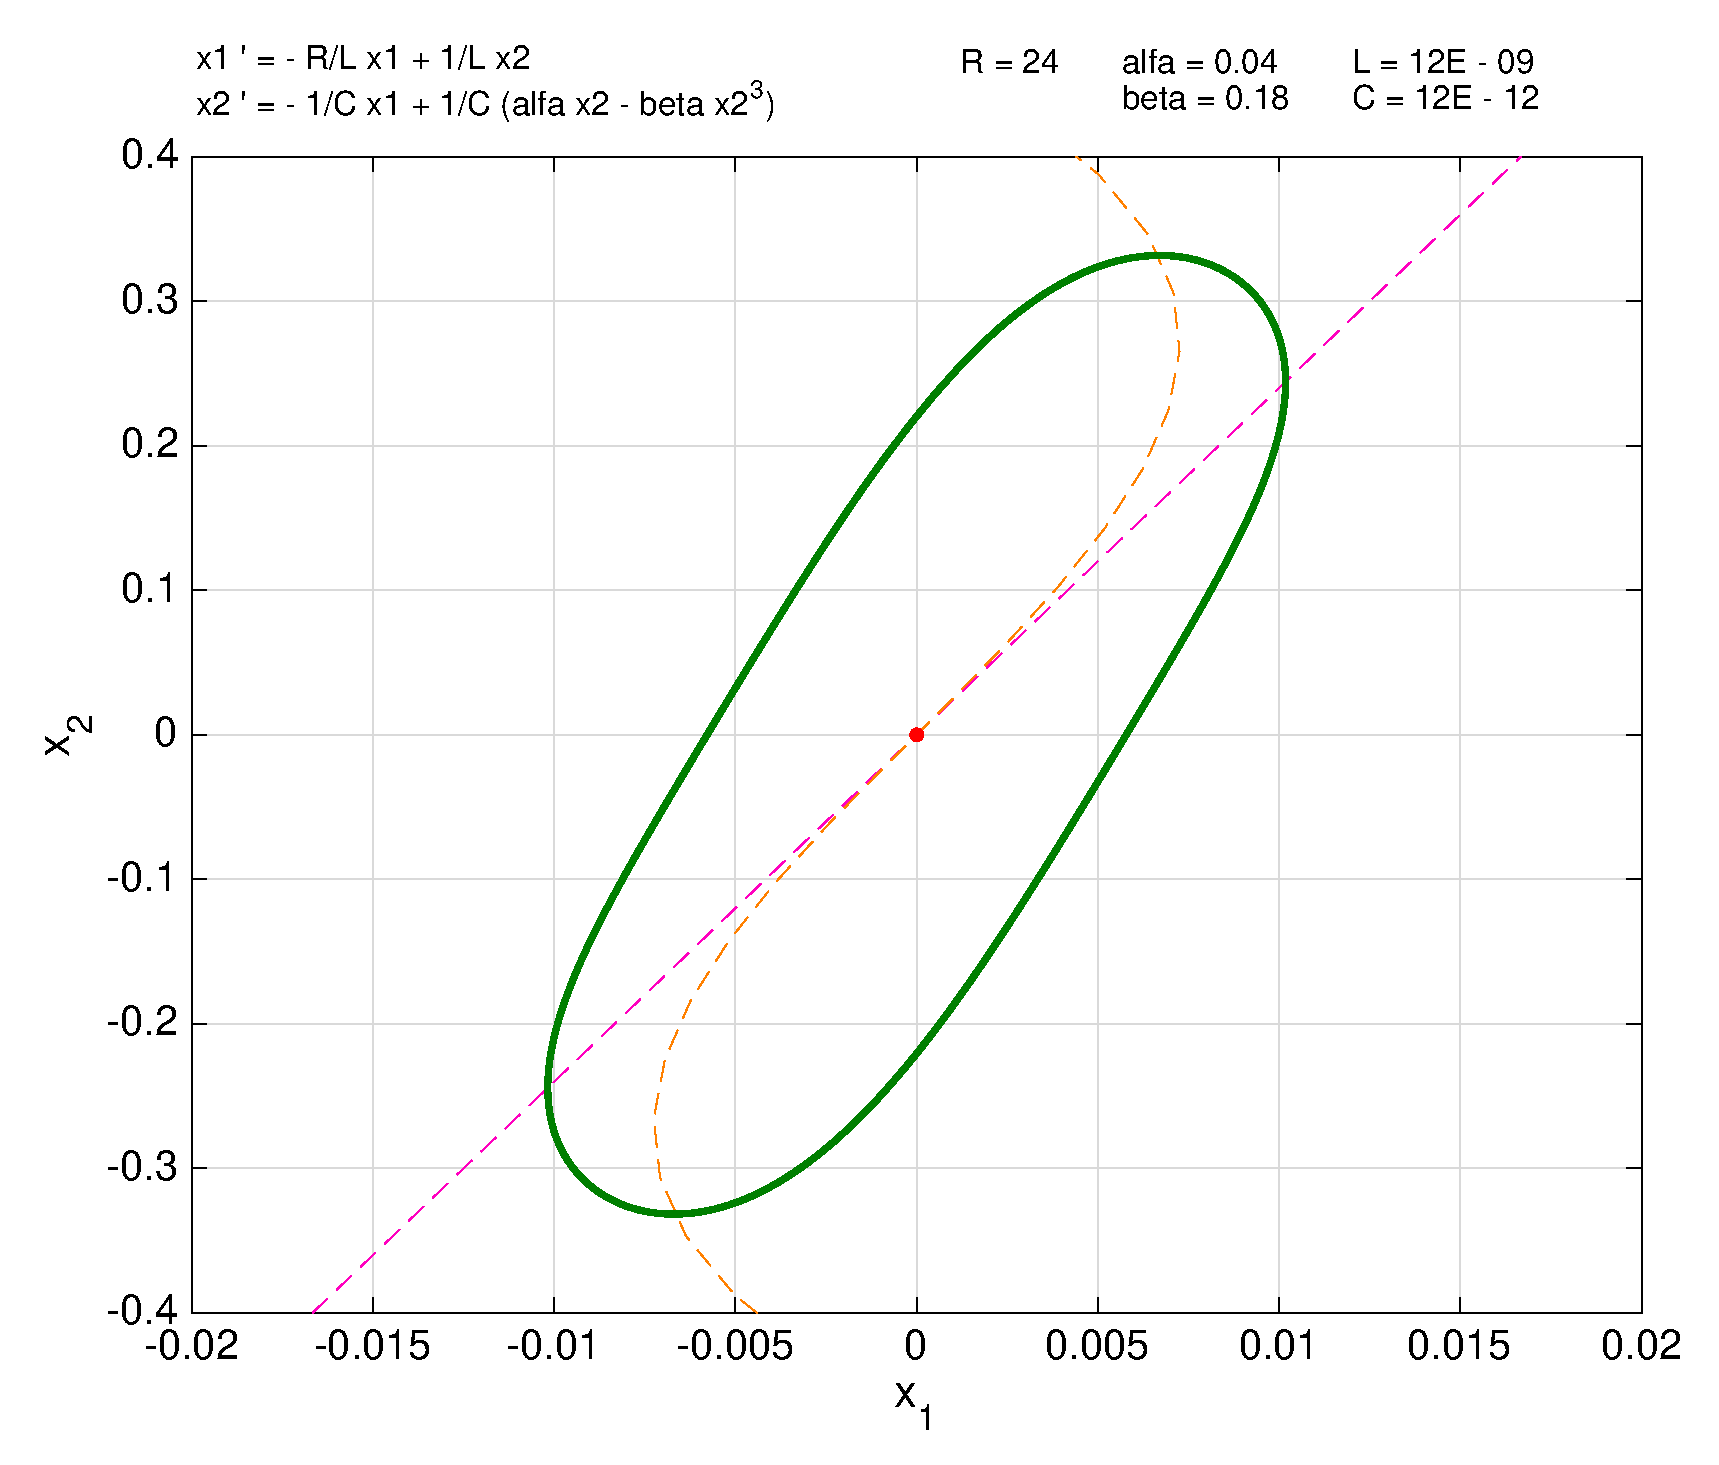
\includegraphics[width=\textwidth]{pplane/Cycle24ohm}
            \caption{Ciclo stabile per $R = 24 \Omega$.}
    \end{subfigure}
    \par\bigskip
    \begin{subfigure}[b]{0.8\textwidth}
            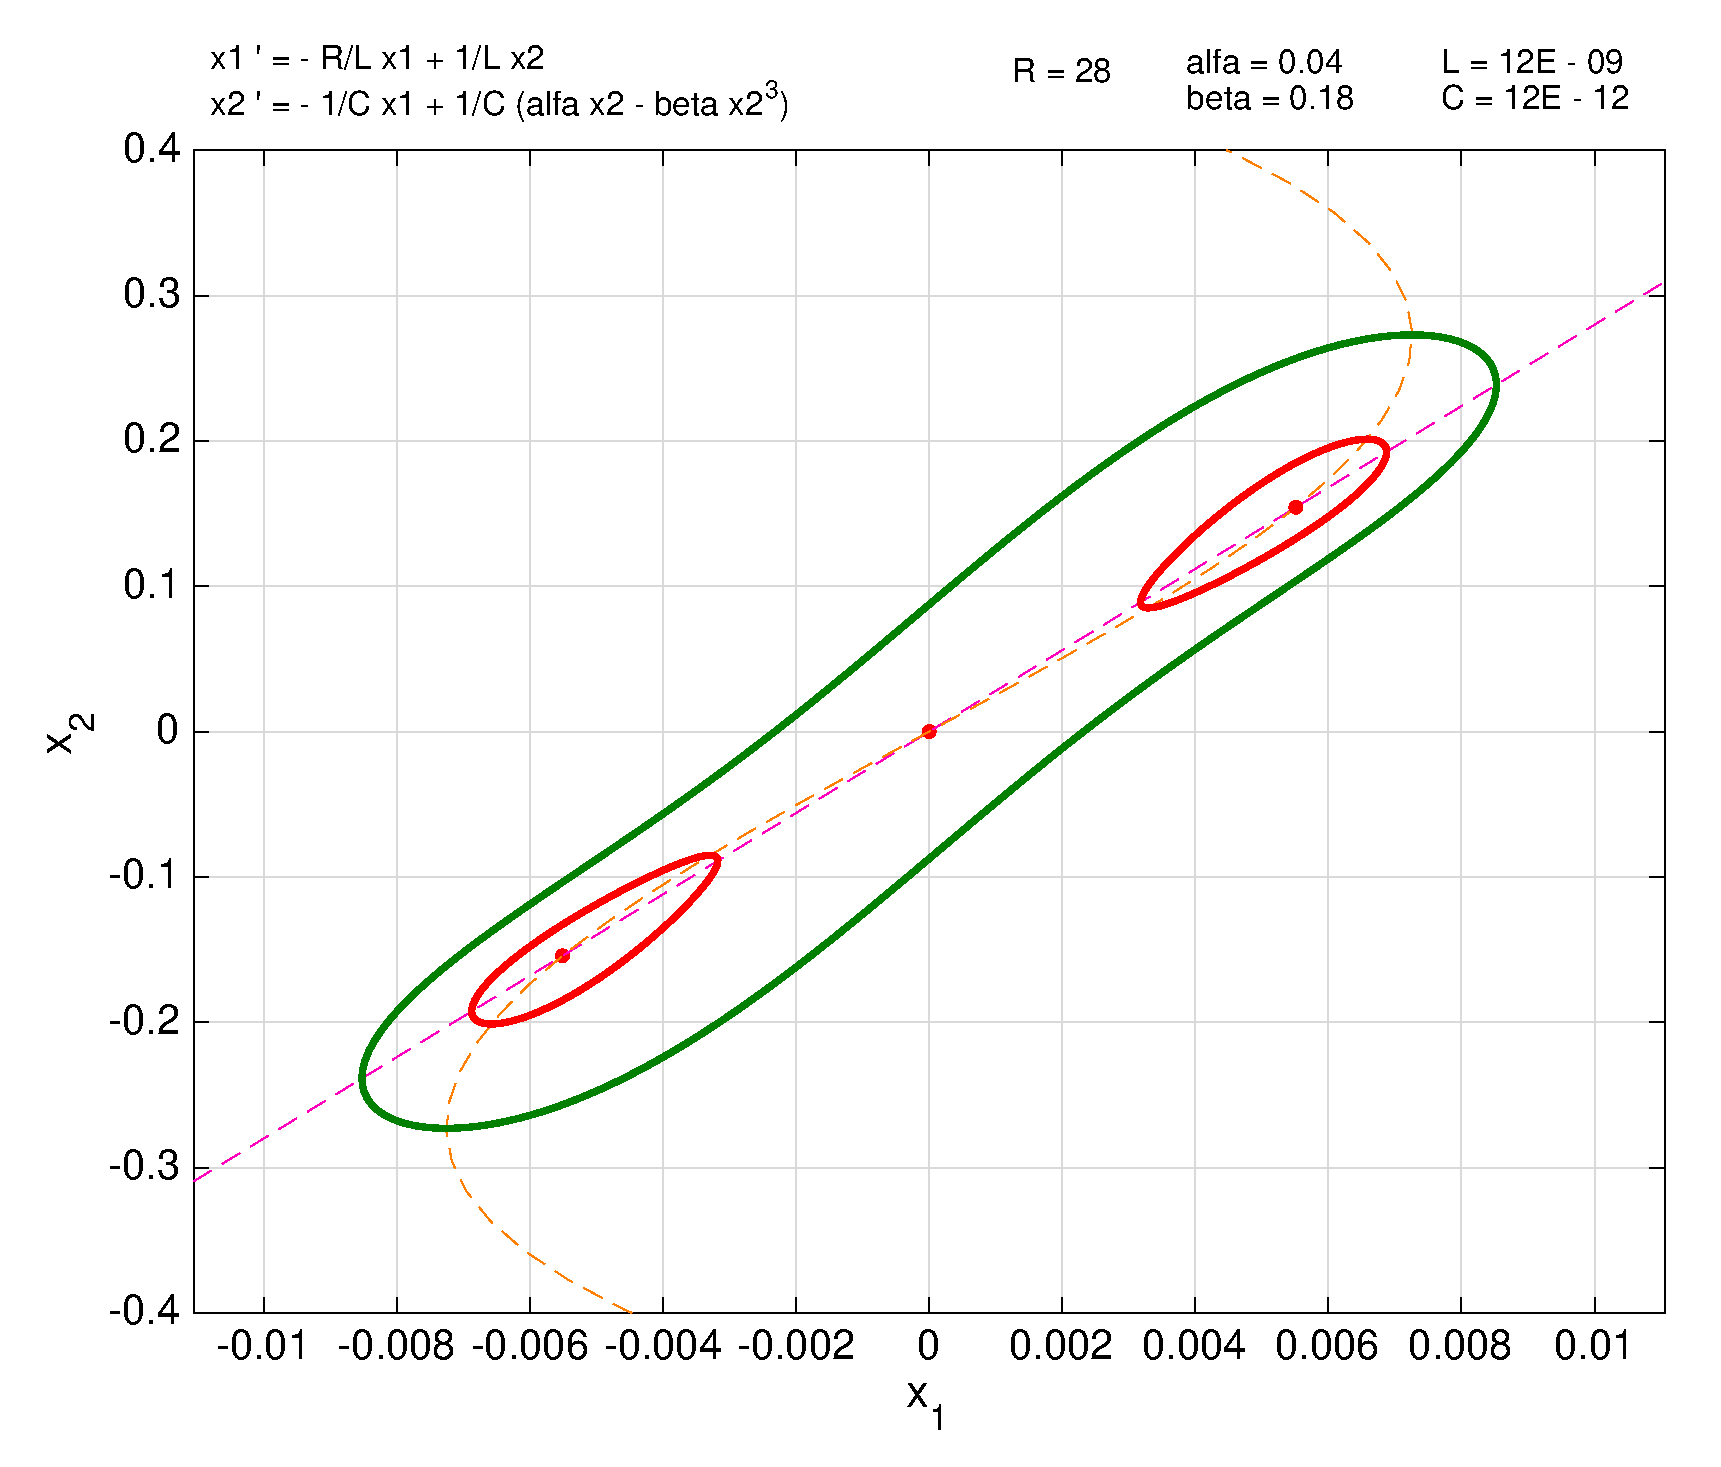
\includegraphics[width=\textwidth]{pplane/Cycle26ohm}
            \caption{Ciclo stabile (esterno) e cicli instabili (interni) per $R = 26 \Omega$.}
            \label{fig:hopf}
    \end{subfigure}
    \caption{Cicli prima e dopo la biforcazione di Hopf.}
    \label{fig:cicli-hopf}
\end{figure}

\begin{figure}
    \centering
    \begin{subfigure}[b]{0.8\textwidth}
            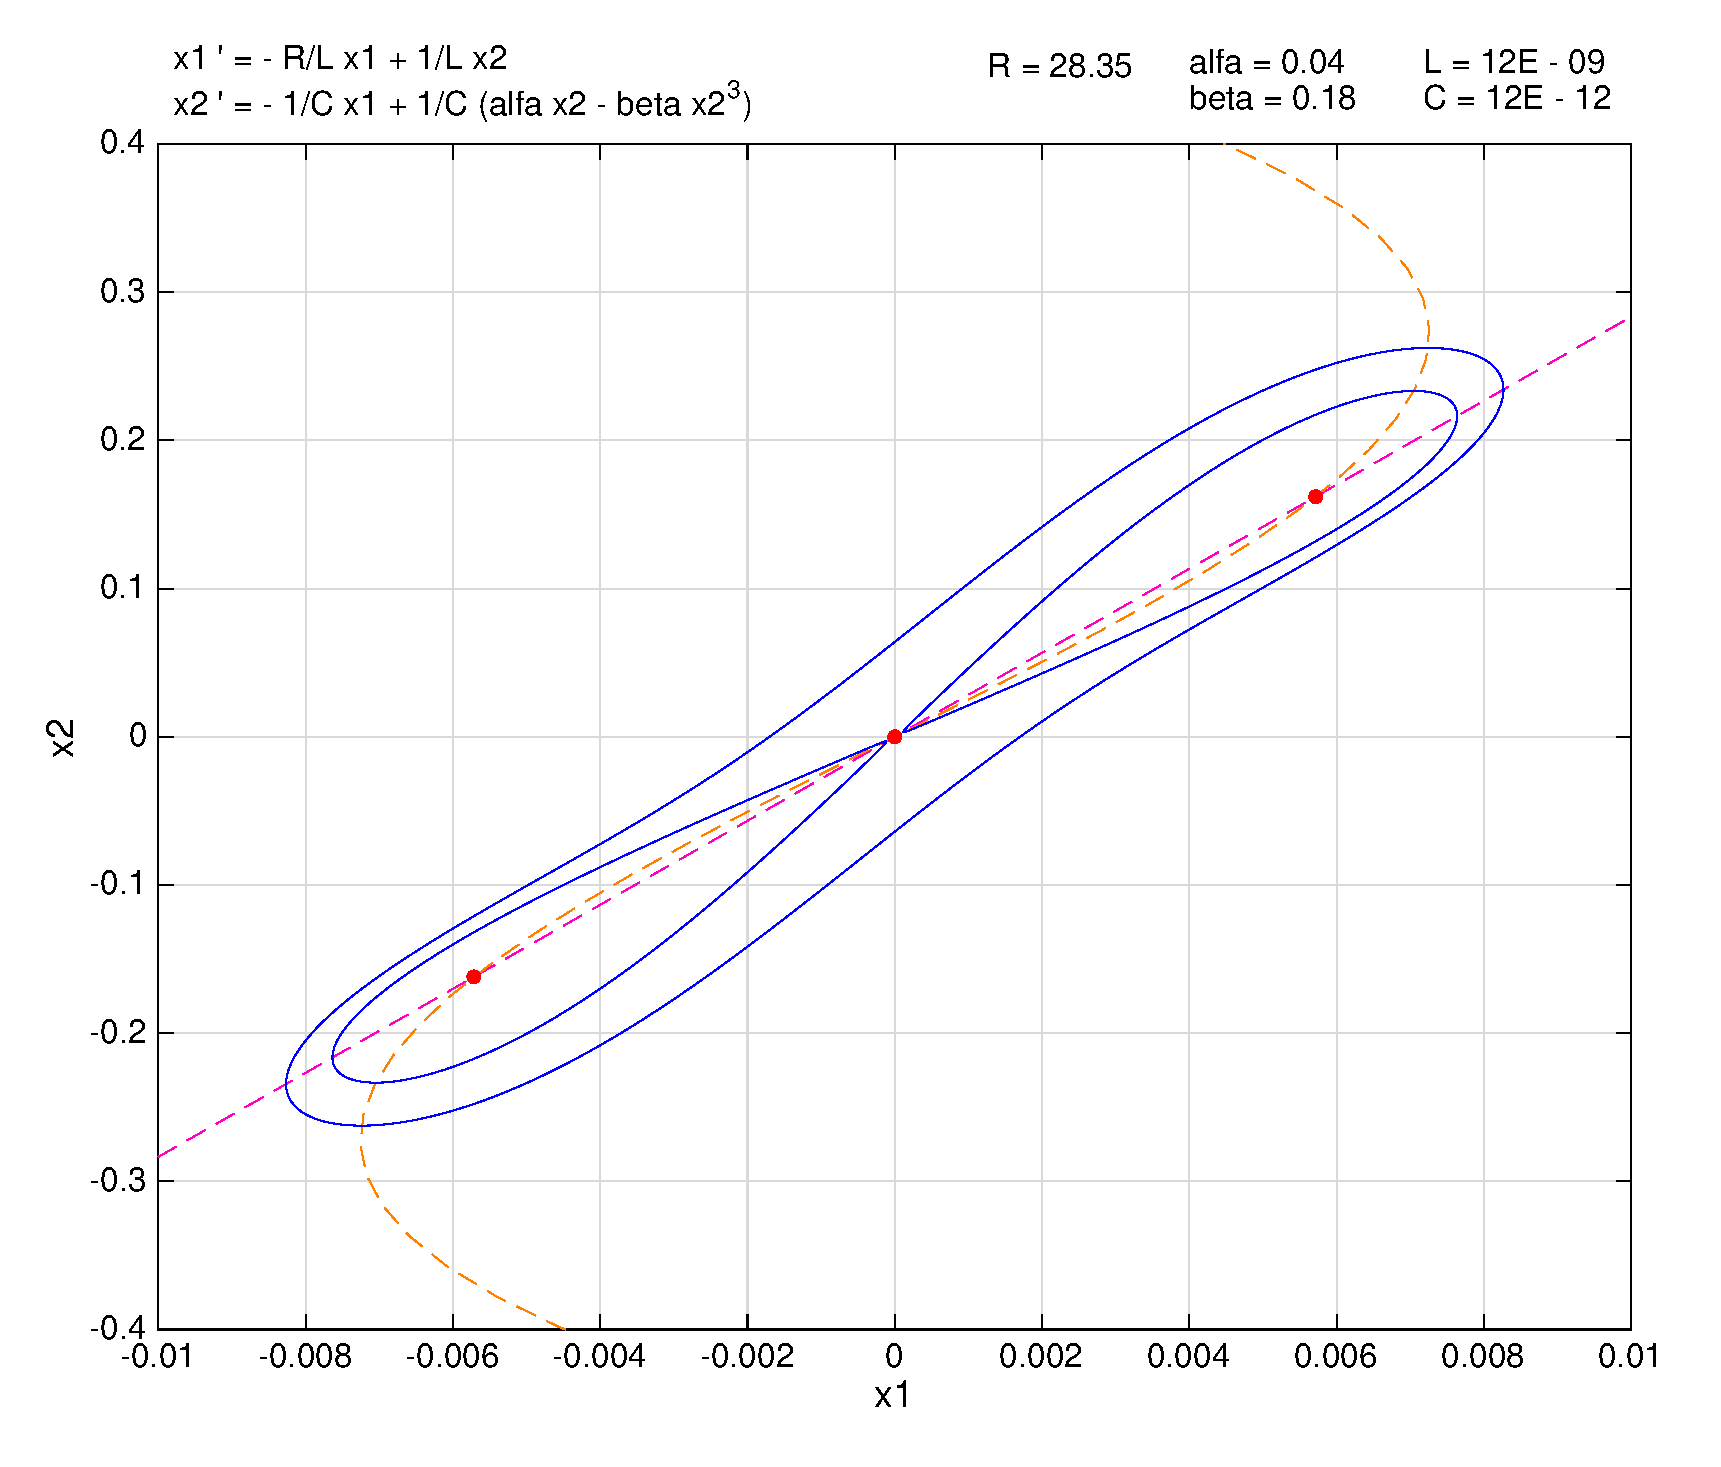
\includegraphics[width=\textwidth]{pplane/DoppiaOmoclina}
            \caption{I due cicli instabili toccano la sella in $(0,0)$ subito prima della biforcazione omoclina.}
    \end{subfigure}
    \par\bigskip
    \begin{subfigure}[b]{0.8\textwidth}
            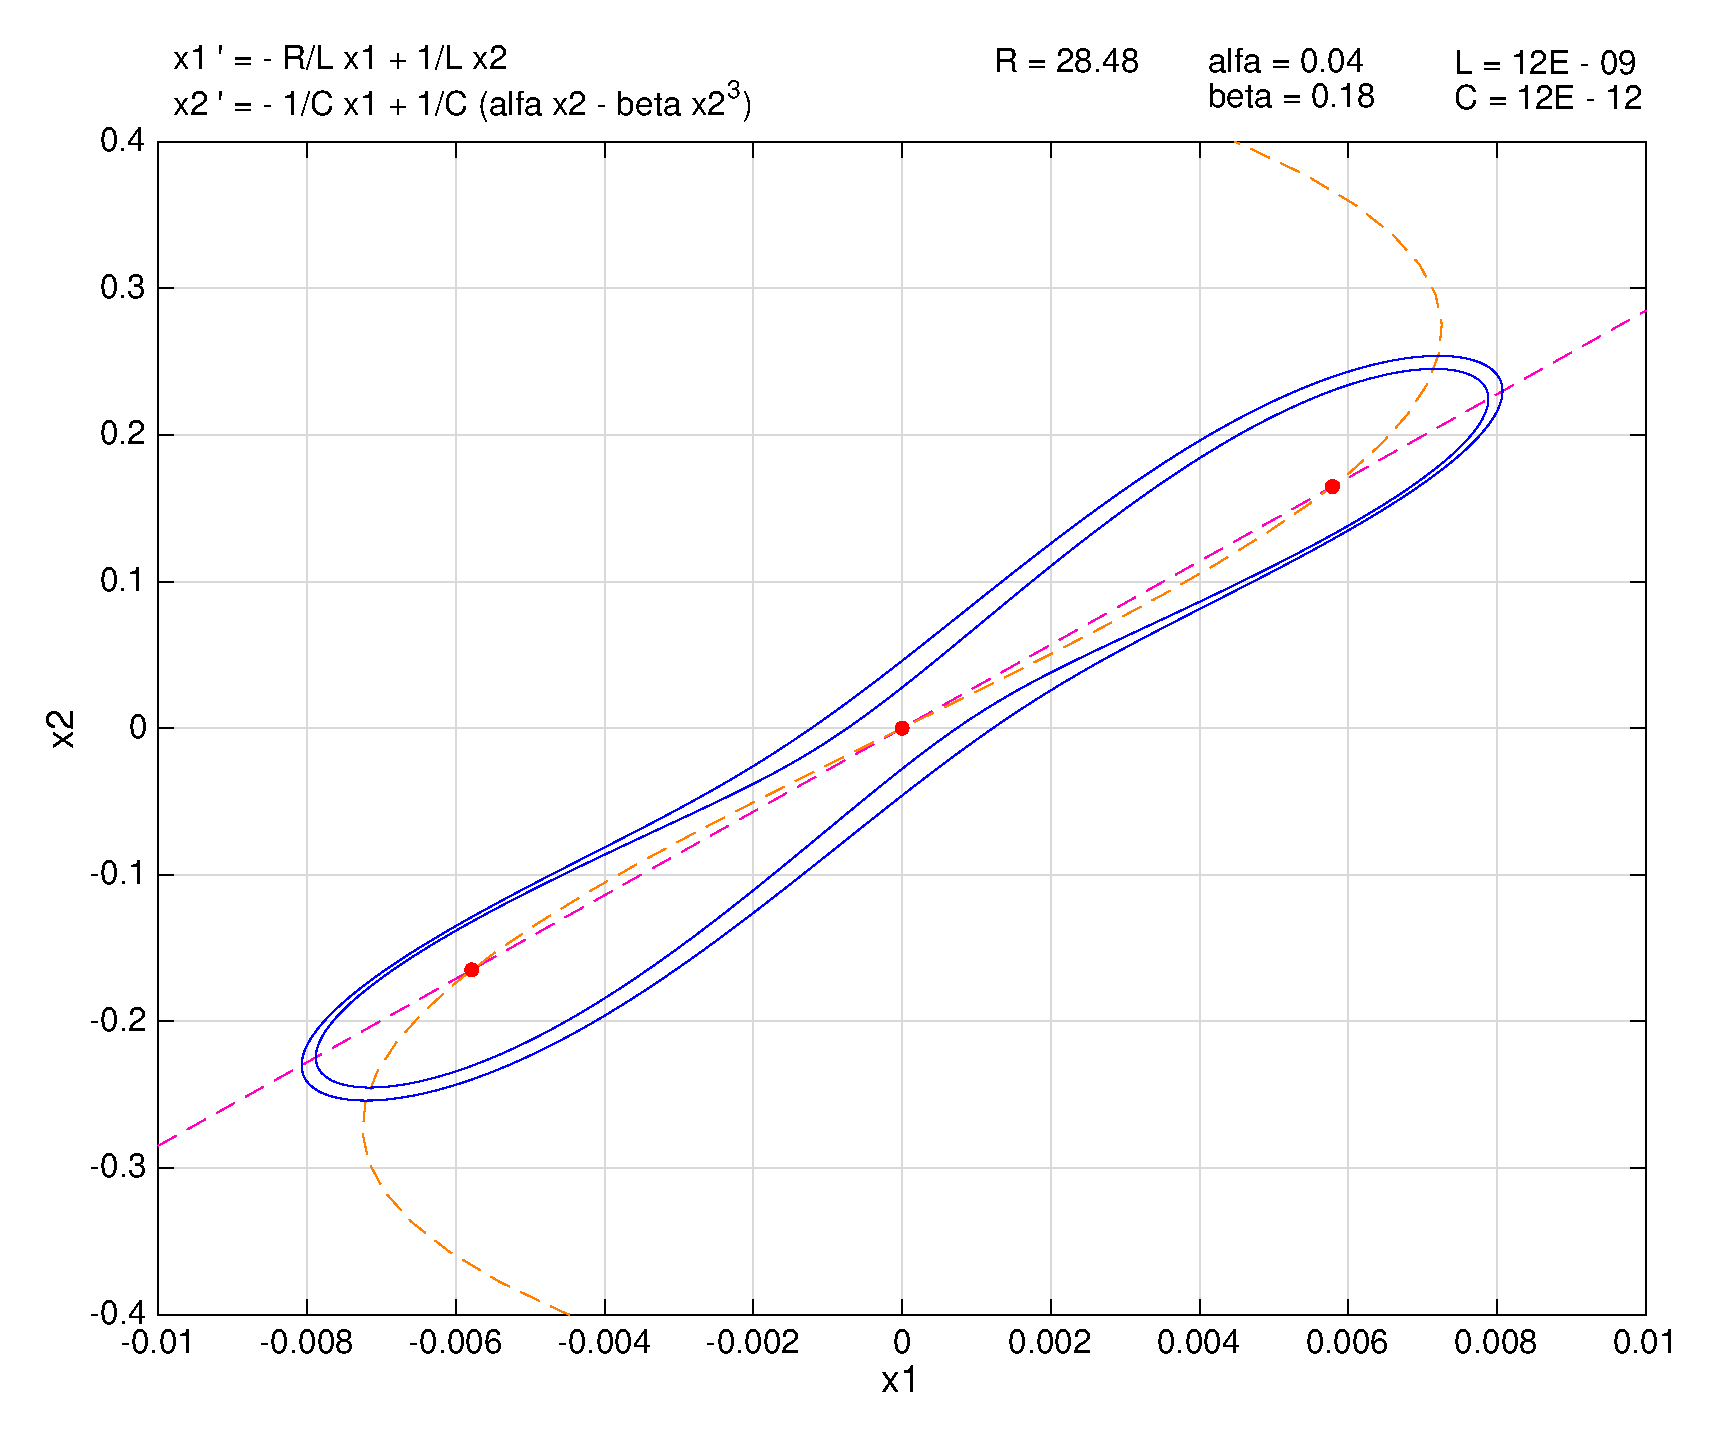
\includegraphics[width=\textwidth]{pplane/TangenteCicli}
            \caption{Dopo la biforcazione omoclina i due cicli instabili si sono fusi; qui sono mostrati immediatamente prima della tangente di cicli.}
            \label{fig:dopo-omoclina}
    \end{subfigure}
    \caption{Cicli prima e dopo la biforcazione omoclina.}
    \label{fig:cicli-omoclina}
\end{figure}
